% !TEX encoding = UTF-8
% !TEX TS-program = pdflatex
% !TEX root = ../Tesi.tex
% !TEX spellcheck = it-IT

%************************************************
\chapter{Modello dei casi d'uso}
\label{cap:modello-casi-d'uso}
%************************************************

Si esegue l'analisi dei casi d'uso nel dominio degli attori che interessano i casi d'uso medesimi suddividendo lo schema completo in sottoschemi, uno per ogni attore, al fine di mantenere una maggior leggibilità del progetto. \\
Si documenta ogni caso d'uso al fine di descrivere nel dettaglio il comportamento del sistema senza riferirsi ad una particolare implementazione.

\section{Attore utente pubblico}
%
% Figura: casi d'uso dell'attore utente pubblico
%
\begin{figure}[h]
	\centering
	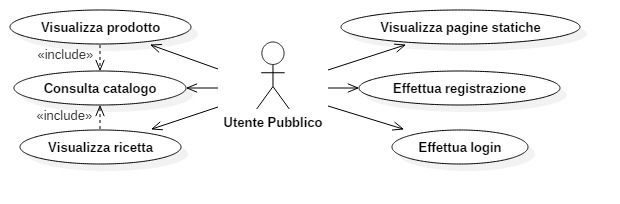
\includegraphics[width=1\textwidth]
	{immagini/attore-utente-pubblico}
	
	\caption{Casi d'uso dell'attore utente pubblico}
\end{figure}

%
% Caso d'uso: Consulta catalogo
%
\subsection{Caso d'uso: Consulta catalogo}

\subsubsection*{Descrizione}
Questa funzionalità permette all'utente pubblico di visualizzare il catalogo dei prodotti navigabile per reparto, caratteristiche, marchio e ricerca libera.

\subsubsection*{Attori coinvolti}
Utente pubblico, partecipazione attiva dell'attore verso il caso d'uso medesimo.

\subsubsection*{Pre-condizioni}
Nessuna precondizione.

\subsubsection*{Post-condizioni}
Nessuna postcondizione, in quanto la consultazione del catalogo non altera lo stato dell'applicazione.

\subsubsection*{Flusso principale}

\begin{enumerate}
	
	\item
	Il form per la ricerca libera e il menù per la consultazione del catalogo per reparti è visibile in tutte le pagine del sito;
	
	\item
	L'utente visualizza tutti i reparti;
	
	\item
	Il sistema visualizza all'utente tutti i reparti;
	
	\item
	L'utente seleziona un reparto;
	
	\item
	Il sistema visualizza all'utente tutti i prodotti dei prodotti che fanno parte del reparto selezionato;
	
	\item
	L'utente seleziona una o più caratteristiche e uno o più marchi per i prodotti di un reparto;
	
	\item
	Il sistema visualizza all'utente i risultati dei prodotti che soddisfano i criteri selezionati.
	
	\item
	L'utente pubblico inserisce del testo nel form per la ricerca libera;
	
	\item
	L'utente pubblico ha la possibilità di scegliere un reparto in cui effettuare una ricerca oppure estendere la ricerca a tutti i reparti;
	
	\item
	L'utente clicca sul pulsante per la ricerca e vengono inviati i dati al server;
	
	\item
	Il sistema effettua la ricerca del testo inserito dall'utente nei vari campi della tabella dei prodotti della base dati;
	
	\item
	Il sistema visualizza la tabella dei prodotti che soddisfano i campi della ricerca, ovvero fanno parte della tabella tutti i prodotti che contengono nei loro campi almeno una ricorrenza del testo da ricercare; 
	
	\item
	L'utente può raffinare la ricerca selezionando una o più caratteristiche e uno o più marchi per i prodotti di un reparto;
	
\end{enumerate}

\subsubsection*{Flussi alternativi}
Non presenti.

%
% Caso d'uso: Visualizza pagine statiche
%
\subsection{Caso d'uso: Visualizza pagine statiche}

	\subsubsection*{Descrizione}
	Questa funzionalità permette all'utente pubblico di visualizzare tutte le pagine richieste con contenuto non dinamico.
	
	\subsubsection*{Attori coinvolti}
	Utente pubblico, partecipazione attiva, richiedendo la visualizzazione delle pagine.
	
	\subsubsection*{Pre-condizioni}
	Nessuna precondizione, in quanto non serve uno stato particolare per visualizzare una pagina statica.
	
	\subsubsection*{Post-condizioni}
	Nessuna postcondizione, in quanto la visualizzazione di una pagina statica non altera lo stato dell'applicazione.
	
	\subsubsection*{Flusso principale}
	
	\begin{enumerate}
		
		\item
		Richiesta di qualsiasi pagina che abbia contenuto statico da parte dell'utente pubblico
		
		\item
		Risposta del server con la pagina statica richiesta da parte dell'utente pubblico;
		
	\end{enumerate}
	
	\subsubsection*{Flussi alternativi}
	Non presenti.

%
% Caso d'uso: Effettua registrazione
%
\subsection{Caso d'uso: Effettua registrazione}

	\subsubsection*{Descrizione}
	Questa funzionalità permette di registrare l'utente all'interno del database, consentendogli tutte le operazioni dell'utente registrato.
	
	\subsubsection*{Attori coinvolti}
	Utente pubblico, partecipazione attiva dell'attore verso il caso d'uso medesimo.
	
	\subsubsection*{Pre-condizioni}
	Nessuna precondizione.
	
	\subsubsection*{Post-condizioni}
	Viene aggiornato lo stato sul database con l'inserimento di un nuovo utente.
	
	\subsubsection*{Flusso principale}
	
		\begin{enumerate}
			
			\item
			L'utente visualizza il form da compilare per effettuare la registrazione nel sistema;
			
			\item
			L'utente compila tutti i campi visualizzati nel modulo con controllo diretto se i dati inseriti sono sintatticamente corretti oppure no;
			
			\item
			L'utente capisce che il dato inserito è sbagliato se il campo dove ha inserito l'informazione diventa di colore rosso, altrimenti se il colore è inalterato vuol dire che dal punto di vista sintattico le informazioni sono corrette;
			
			\item
			Finché il modulo non è stato inviato al server l'utente può modificare i dati inseriti negli appositi campi di compilazione;
			
			\item
			\label{fcu:effettua-registrazione}
			Quando l'utente richiede l'invio dei dati al server vengono controllati nuovamente tutti i campi del modulo, inoltre è richiesta l'accettazione delle condizioni di utilizzo;
			
			\item
			Una volta che i dati sono stati inviati al server vengono elaborati e memorizzati sul database modificando quindi lo stato del database stesso;
			
			\item
			Viene notificato all'utente l'avvenuto inserimento del proprio profilo nel sistema.
			
		\end{enumerate}
	
	\subsubsection*{Flussi alternativi}
	Nel caso di inserimento di un indirizzo email già esistente nel database, dopo il punto~\ref{fcu:effettua-registrazione} viene visualizzato nuovamente il form precompilato con i dati inseriti nell'ultima compilazione del form, notificando l'utente della presenza nel database di un profilo con lo stesso indirizzo email.

%
% Caso d'uso: Effettua login
%
\subsection{Caso d'uso: Effettua login}

	\subsubsection*{Descrizione}
	Questa funzionalità permette all'utente pubblico di farsi riconoscere dal sistema, accedendo quindi a tutte le sue funzionalità.
	
	\subsubsection*{Attori coinvolti}
	Utente pubblico, partecipazione attiva dell'attore che passa da \emph{Utente Pubblico} a \emph{Utente registrato} o \emph{Utente amministratore} o \emph{Utente super amministratore}.
	
	\subsubsection*{Pre-condizioni}
	Compilazione del modulo di login.
	
	\subsubsection*{Post-condizioni}
	L'utente passa da attore \emph{Utente Pubblico} ad attore \emph{Utente registrato} o ad attore \emph{Utente amministratore} o ad attore \emph{Utente super amministratore}.
	
	\subsubsection*{Flusso principale}
	
	\begin{enumerate}
		
		\item
		Il form per l'autenticazione è visibile in tutte le pagine del sito;
		
		\item
		L'utente pubblico compila il modulo inserendo la propria email e la propria password;
		
		\item
		Il sistema effettua verifica se le informazioni inserite nel campo email sono corrette dal punto di vista sintattico, colorando il campo di colore rosso se l'indirizzo inserito è sbagliato dal punto di vista sintattico;
		
		\item
		L'utente clicca sul pulsante per l'autenticazione e vengono inviati i dati al server;
		
		\item
		Dopo aver ricevuto i dati il server controlla se nella base dati è presente un utente con indirizzo email e password ricevuti;
		
		\item
		Se le informazioni esistono sulla base dati l'utente pubblico viene riconosciuto dal sistema e al posto del form per l'autenticazione viene visualizzato il nome dell'utente e un menù con tutte le operazioni che l'utente può eseguire sul sistema.
		
	\end{enumerate}
	
	\subsubsection*{Flussi alternativi}
	Nel caso di inserimento di email e password non presenti nel database vengono notificate all'utente pubblico le possibili cause di errore.

\section{Attore utente registrato}
%
% Figura: casi d'uso dell'attore utente registrato
%
\begin{figure}[h]
	\centering
	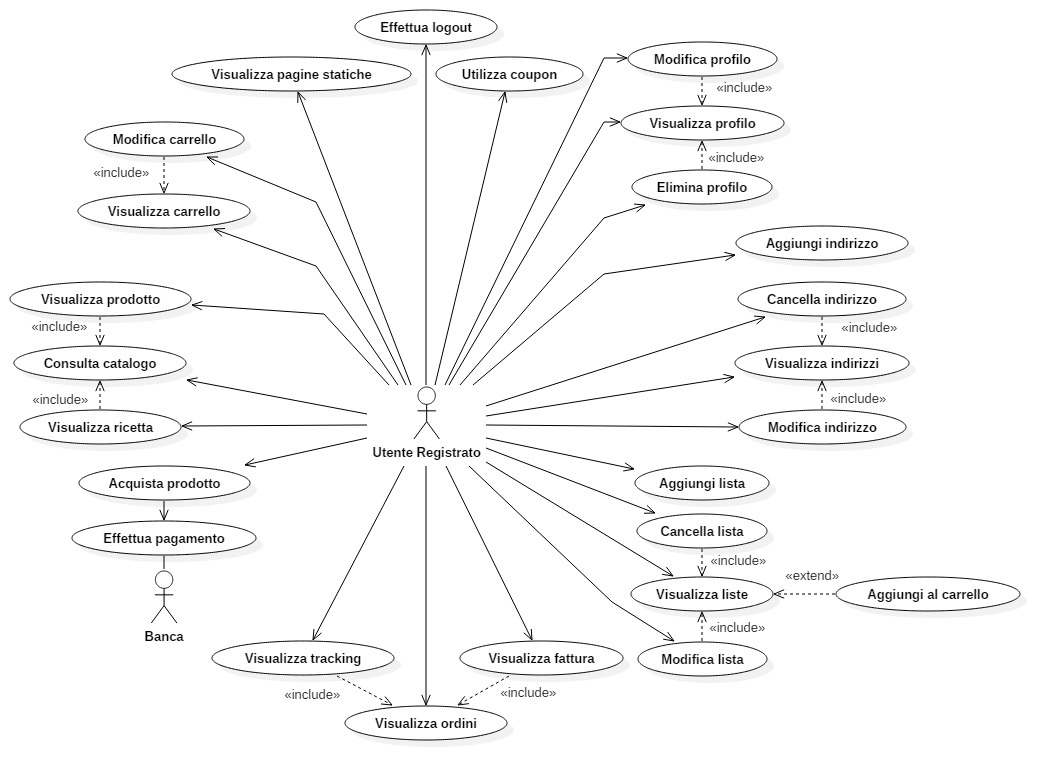
\includegraphics[width=1\textwidth]
	{immagini/attore-utente-registrato}
	
	\caption{Casi d'uso dell'attore utente registrato}
\end{figure}

\section{Attore utente super amministratore}
%
% Figura: casi d'uso dell'attore utente super amministratore
%
\begin{figure}[h]
	\centering
	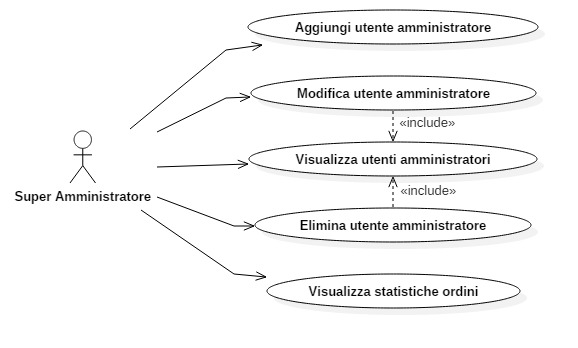
\includegraphics[width=1\textwidth]
	{immagini/attore-utente-super-amministratore}
	
	\caption{Casi d'uso dell'attore utente super amministratore}
\end{figure}

\section{Attore utente amministratore}
%
% Figura: casi d'uso dell'attore utente amministratore
%
\begin{figure}[h]
	\centering
	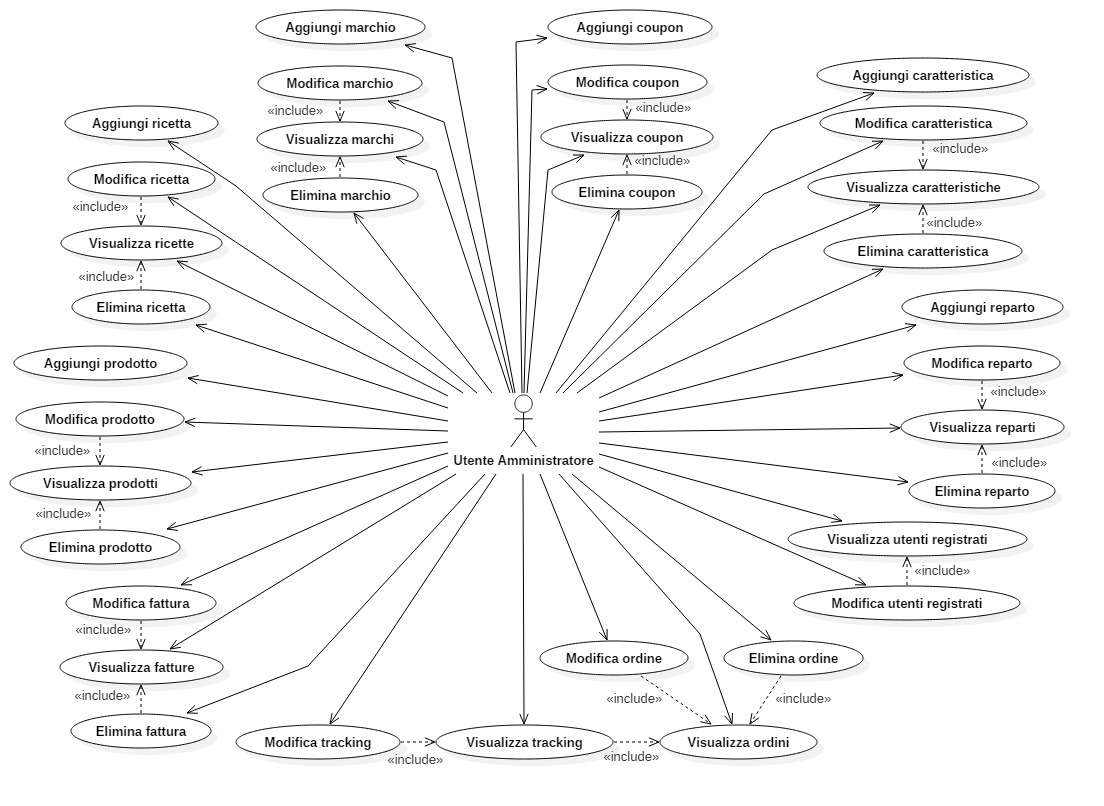
\includegraphics[width=1\textwidth]
	{immagini/attore-utente-amministratore}
	
	\caption{Casi d'uso dell'attore utente amministratore}
\end{figure}

\section{Diagramma delle attività}
\begin{enumerate}
	\item
	Consultazione catalogo
	
	\item
	Acquisto di un prodotto
	
\end{enumerate}